\documentclass{standalone}
\usepackage{tikz}
\usetikzlibrary{patterns, positioning}

\begin{document}
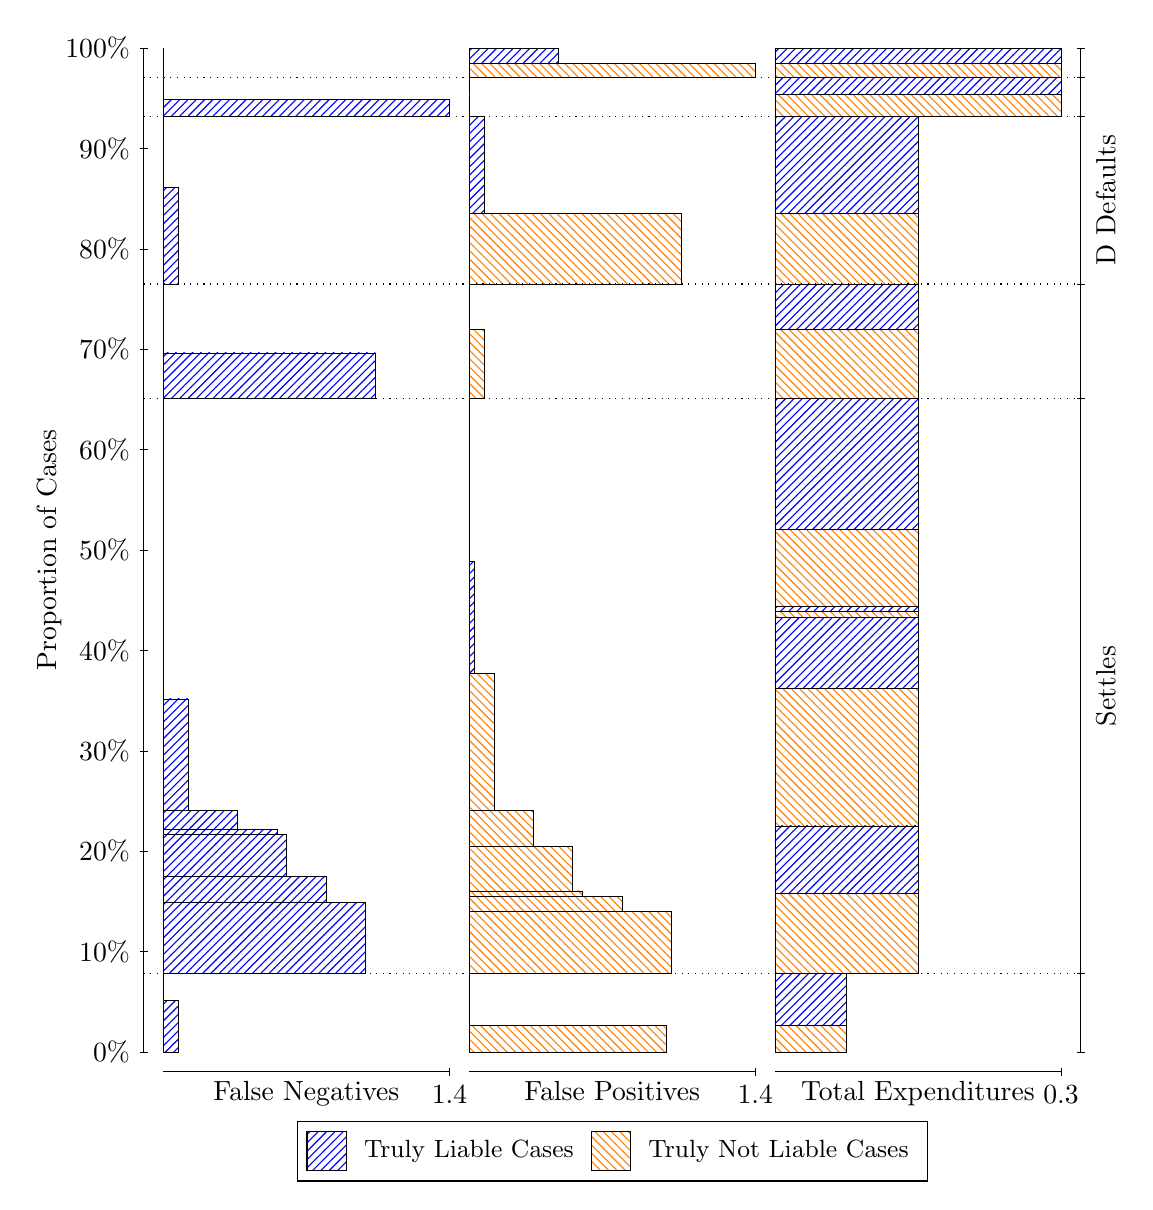
\begin{tikzpicture}
\draw[black, very thin] (1.5,1.75) -- (1.5,14.5);
\node[rotate=90, anchor=center] at (0.3, 8.125) {Proportion of Cases};
\draw[black, very thin] (1.45,1.75) -- (1.55,1.75);
\node[anchor=east] at (1.45, 1.75) {0\%};
\draw[black, very thin] (1.45,3.025) -- (1.55,3.025);
\node[anchor=east] at (1.45, 3.025) {10\%};
\draw[black, very thin] (1.45,4.3) -- (1.55,4.3);
\node[anchor=east] at (1.45, 4.3) {20\%};
\draw[black, very thin] (1.45,5.575) -- (1.55,5.575);
\node[anchor=east] at (1.45, 5.575) {30\%};
\draw[black, very thin] (1.45,6.85) -- (1.55,6.85);
\node[anchor=east] at (1.45, 6.85) {40\%};
\draw[black, very thin] (1.45,8.125) -- (1.55,8.125);
\node[anchor=east] at (1.45, 8.125) {50\%};
\draw[black, very thin] (1.45,9.4) -- (1.55,9.4);
\node[anchor=east] at (1.45, 9.4) {60\%};
\draw[black, very thin] (1.45,10.675) -- (1.55,10.675);
\node[anchor=east] at (1.45, 10.675) {70\%};
\draw[black, very thin] (1.45,11.95) -- (1.55,11.95);
\node[anchor=east] at (1.45, 11.95) {80\%};
\draw[black, very thin] (1.45,13.225) -- (1.55,13.225);
\node[anchor=east] at (1.45, 13.225) {90\%};
\draw[black, very thin] (1.45,14.5) -- (1.55,14.5);
\node[anchor=east] at (1.45, 14.5) {100\%};

\draw[black, very thin] (13.4,1.75) -- (13.4,14.5);
\draw[black, very thin] (13.35,1.75) -- (13.45,1.75);
\node[anchor=west] at (13.35, 1.75) {};
\draw[black, very thin] (13.35,2.7449) -- (13.45,2.7449);
\node[anchor=west] at (13.35, 2.7449) {};
\draw[black, very thin] (13.35,10.048) -- (13.45,10.048);
\node[anchor=west] at (13.35, 10.048) {};
\draw[black, very thin] (13.35,11.503) -- (13.45,11.503);
\node[anchor=west] at (13.35, 11.503) {};
\draw[black, very thin] (13.35,13.633) -- (13.45,13.633);
\node[anchor=west] at (13.35, 13.633) {};
\draw[black, very thin] (13.35,14.123) -- (13.45,14.123);
\node[anchor=west] at (13.35, 14.123) {};
\draw[black, very thin] (13.35,14.5) -- (13.45,14.5);
\node[anchor=west] at (13.35, 14.5) {};

\draw[black, very thin, pattern color=blue, pattern=north east lines] (1.75,1.75) rectangle (1.9379,2.4091);
\draw[black, very thin, pattern color=orange, pattern=north west lines] (1.75,2.4091) rectangle (1.75,2.7449);
\draw[black, very thin, pattern color=blue, pattern=north east lines] (1.75,2.7449) rectangle (4.3184,3.6541);
\draw[black, very thin, pattern color=blue, pattern=north east lines] (1.75,3.6541) rectangle (3.8172,3.9756);
\draw[black, very thin, pattern color=blue, pattern=north east lines] (1.75,3.9756) rectangle (3.3161,4.5105);
\draw[black, very thin, pattern color=blue, pattern=north east lines] (1.75,4.5105) rectangle (3.1908,4.5754);
\draw[black, very thin, pattern color=blue, pattern=north east lines] (1.75,4.5754) rectangle (2.6897,4.815);
\draw[black, very thin, pattern color=blue, pattern=north east lines] (1.75,4.815) rectangle (2.0632,6.2347);
\draw[black, very thin, pattern color=orange, pattern=north west lines] (1.75,6.2347) rectangle (1.75,10.048);
\draw[black, very thin, pattern color=blue, pattern=north east lines] (1.75,10.048) rectangle (4.4437,10.627);
\draw[black, very thin, pattern color=orange, pattern=north west lines] (1.75,10.627) rectangle (1.75,11.503);
\draw[black, very thin, pattern color=blue, pattern=north east lines] (1.75,11.503) rectangle (1.9379,12.735);
\draw[black, very thin, pattern color=orange, pattern=north west lines] (1.75,12.735) rectangle (1.75,13.633);
\draw[black, very thin, pattern color=blue, pattern=north east lines] (1.75,13.633) rectangle (5.3833,13.847);
\draw[black, very thin, pattern color=orange, pattern=north west lines] (1.75,13.847) rectangle (1.75,14.123);
\draw[black, very thin, pattern color=orange, pattern=north west lines] (1.75,14.123) rectangle (1.75,14.3);
\draw[black, very thin, pattern color=blue, pattern=north east lines] (1.75,14.3) rectangle (1.75,14.5);
\draw[black, very thin, pattern color=orange, pattern=north west lines] (5.6333,1.75) rectangle (8.1391,2.0858);
\draw[black, very thin, pattern color=blue, pattern=north east lines] (5.6333,2.0858) rectangle (5.6333,2.7449);
\draw[black, very thin, pattern color=orange, pattern=north west lines] (5.6333,2.7449) rectangle (8.2017,3.5384);
\draw[black, very thin, pattern color=orange, pattern=north west lines] (5.6333,3.5384) rectangle (7.5753,3.7272);
\draw[black, very thin, pattern color=orange, pattern=north west lines] (5.6333,3.7272) rectangle (7.0741,3.7954);
\draw[black, very thin, pattern color=orange, pattern=north west lines] (5.6333,3.7954) rectangle (6.9489,4.3595);
\draw[black, very thin, pattern color=orange, pattern=north west lines] (5.6333,4.3595) rectangle (6.4477,4.8147);
\draw[black, very thin, pattern color=orange, pattern=north west lines] (5.6333,4.8147) rectangle (5.9466,6.5581);
\draw[black, very thin, pattern color=blue, pattern=north east lines] (5.6333,6.5581) rectangle (5.696,7.9779);
\draw[black, very thin, pattern color=blue, pattern=north east lines] (5.6333,7.9779) rectangle (5.6333,10.048);
\draw[black, very thin, pattern color=orange, pattern=north west lines] (5.6333,10.048) rectangle (5.8213,10.924);
\draw[black, very thin, pattern color=blue, pattern=north east lines] (5.6333,10.924) rectangle (5.6333,11.503);
\draw[black, very thin, pattern color=orange, pattern=north west lines] (5.6333,11.503) rectangle (8.327,12.4);
\draw[black, very thin, pattern color=blue, pattern=north east lines] (5.6333,12.4) rectangle (5.8213,13.633);
\draw[black, very thin, pattern color=orange, pattern=north west lines] (5.6333,13.633) rectangle (5.6333,13.908);
\draw[black, very thin, pattern color=blue, pattern=north east lines] (5.6333,13.908) rectangle (5.6333,14.123);
\draw[black, very thin, pattern color=orange, pattern=north west lines] (5.6333,14.123) rectangle (9.2667,14.3);
\draw[black, very thin, pattern color=blue, pattern=north east lines] (5.6333,14.3) rectangle (6.7609,14.5);
\draw[black, very thin, pattern color=orange, pattern=north west lines] (9.5167,1.75) rectangle (10.425,2.0858);
\draw[black, very thin, pattern color=blue, pattern=north east lines] (9.5167,2.0858) rectangle (10.425,2.7449);
\draw[black, very thin, pattern color=orange, pattern=north west lines] (9.5167,2.7449) rectangle (11.333,3.7642);
\draw[black, very thin, pattern color=blue, pattern=north east lines] (9.5167,3.7642) rectangle (11.333,4.6206);
\draw[black, very thin, pattern color=orange, pattern=north west lines] (9.5167,4.6206) rectangle (11.333,6.364);
\draw[black, very thin, pattern color=blue, pattern=north east lines] (9.5167,6.364) rectangle (11.333,7.2733);
\draw[black, very thin, pattern color=orange, pattern=north west lines] (9.5167,7.2733) rectangle (11.333,7.3415);
\draw[black, very thin, pattern color=blue, pattern=north east lines] (9.5167,7.3415) rectangle (11.333,7.4063);
\draw[black, very thin, pattern color=orange, pattern=north west lines] (9.5167,7.4063) rectangle (11.333,8.3886);
\draw[black, very thin, pattern color=blue, pattern=north east lines] (9.5167,8.3886) rectangle (11.333,10.048);
\draw[black, very thin, pattern color=orange, pattern=north west lines] (9.5167,10.048) rectangle (11.333,10.924);
\draw[black, very thin, pattern color=blue, pattern=north east lines] (9.5167,10.924) rectangle (11.333,11.503);
\draw[black, very thin, pattern color=orange, pattern=north west lines] (9.5167,11.503) rectangle (11.333,12.4);
\draw[black, very thin, pattern color=blue, pattern=north east lines] (9.5167,12.4) rectangle (11.333,13.633);
\draw[black, very thin, pattern color=orange, pattern=north west lines] (9.5167,13.633) rectangle (13.15,13.908);
\draw[black, very thin, pattern color=blue, pattern=north east lines] (9.5167,13.908) rectangle (13.15,14.123);
\draw[black, very thin, pattern color=orange, pattern=north west lines] (9.5167,14.123) rectangle (13.15,14.3);
\draw[black, very thin, pattern color=blue, pattern=north east lines] (9.5167,14.3) rectangle (13.15,14.5);
\draw[black, dotted] (1.5,2.7449) -- (13.4,2.7449);
\draw[black, dotted] (1.5,10.048) -- (13.4,10.048);
\draw[black, dotted] (1.5,11.503) -- (13.4,11.503);
\draw[black, dotted] (1.5,13.633) -- (13.4,13.633);
\draw[black, dotted] (1.5,14.123) -- (13.4,14.123);
\draw[black, very thin] (1.75,1.5) -- (5.3833,1.5);
\node[anchor=north] at (3.5667, 1.5) {False Negatives};
\draw[black, very thin] (5.3833,1.45) -- (5.3833,1.55);
\node[anchor=north] at (5.3833, 1.45) {1.4};

\draw[black, very thin] (5.6333,1.5) -- (9.2667,1.5);
\node[anchor=north] at (7.45, 1.5) {False Positives};
\draw[black, very thin] (9.2667,1.45) -- (9.2667,1.55);
\node[anchor=north] at (9.2667, 1.45) {1.4};

\draw[black, very thin] (9.5167,1.5) -- (13.15,1.5);
\node[anchor=north] at (11.333, 1.5) {Total Expenditures};
\draw[black, very thin] (13.15,1.45) -- (13.15,1.55);
\node[anchor=north] at (13.15, 1.45) {0.3};


\node[black, centered, rotate=90] at (13.72, 6.3964) {Settles};

\node[black, centered, rotate=90] at (13.72, 12.568) {D Defaults};



\draw (7.449999999999999,1.5) node[draw=none] (baseCoordinate) {};
\begin{scope}[align=center]
        \matrix[scale=0.5, draw=black, below=0.5cm of baseCoordinate, nodes={draw}, column sep=0.1cm]{
            \node[rectangle, draw, minimum width=0.5cm, minimum height=0.5cm, pattern=north east lines, pattern color=blue] {}; &
            \node[draw=none, font=\small] (B) {Truly Liable Cases}; &
            \node[rectangle, draw, minimum width=0.5cm, minimum height=0.5cm, pattern=north west lines, pattern color=orange] {}; &
            \node[draw=none, font=\small] (B) {Truly Not Liable Cases}; \\
            };
\end{scope}

\end{tikzpicture}
\end{document}